\chapter{Einzelansicht Mitglied}\label{personal:person}
Das Fenster in \cref{fig:personal:person} zeigt das Standardfenster für die Bearbeitung der Personendaten.
Im Kopf werden der Name und die Mitgliedsnummer angezeigt und können geändert werden.
Beim Erstellen einer Person wird automatisch, die nächsthöhere Mitgliedsnummer vergeben, als aktuell vorhanden.
Ein Ändern der Mitgliedsnummer ist nur möglich, wenn die Nummer nicht bereits vergeben ist.

Für juristische Personen, die als Fördermitglieder aufgenommen sind, kann der Vorname freigelassen werden.
Es genügt hierbei den Nachnamen anzugeben.

\begin{figure}[!h]
  \centering
	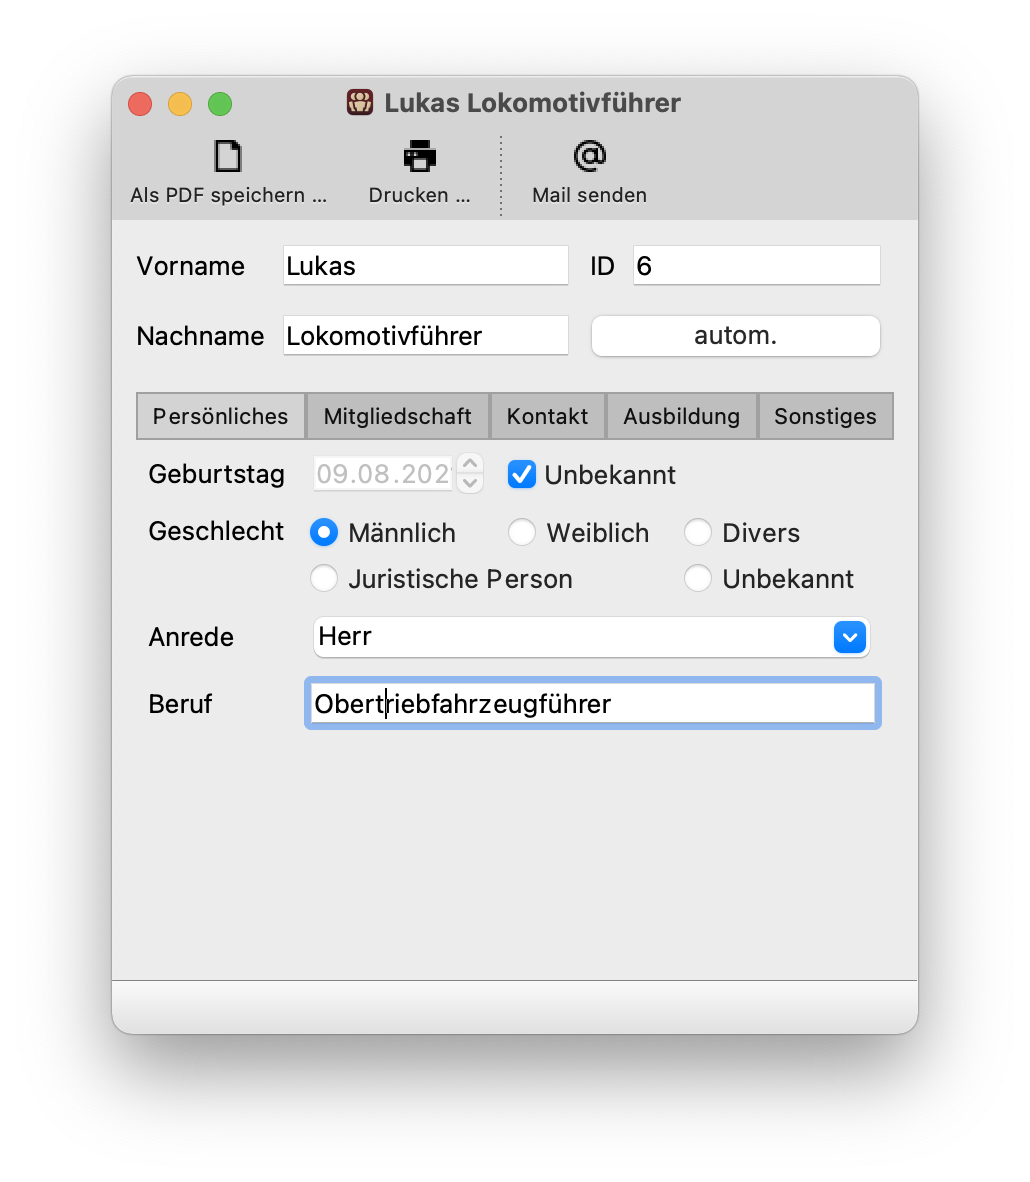
\includegraphics[width=0.75\textwidth]{img/personal-person}
	\caption{Das Fenster zum Bearbeiten der Daten eines Mitglieds.}
	\label{fig:personal:person}
\end{figure}


Im unteren Bereich des Fensters stehen verschiedene Reiter zur Verfügung,
über welche die persönlichen Daten abgerufen und verändert werden können.


\paragraph{Person Löschen}
Sie können über das Menü \aktion{Person} die Person aus dem System entfernen.
Dies ist nur möglich, wenn sie bei keiner Aktivität mehr eingetragen ist.
Ist eine Person aus dem Verein ausgetreten, ist es \textbf{nicht} erforderlich sie zu löschen.
Stattdessen kann die Person als ausgetreten markiert und das Austrittsdatum vermerkt werden.
Somit bleibt die Person weiterhin im System erhalten und wird auch bei den jeweiligen Aktivitäten noch mit ausgegeben.


\paragraph{Betriebsdienst}
Für den Betriebsdienst kann eine Datum eingegeben werden, dass beschreibt bis wann die betriebliche Tauglichkeitsuntersuchung gültig ist.
Liegt für den Tag einer Aktivität keine Tauglichkeit vor, kann die Person nicht in der entsprechenden Kategorie eingetragen werden (z.B.\ als Tf oder Zf).
Für Zugbegleiter wird dann automatisch eine Eintragung als Begl.o.b.A.\ eingetragen.


\paragraph{Export}
Über das Menü \aktion{Export} kann das Stammdatenblatt der geöffneten Person exportiert werden.
Das Dokument enthält alle personenbezogenen Daten aus der EPL-Datei.
Es enthält jedoch keine Informationen zu Aktivitäten und geleisteten Stunden.
